\documentclass[12pt]{article}
\title{ECE 141 Homework 4}
\usepackage{subcaption}
\author{Lawrence Liu}
\usepackage{graphicx}
\usepackage{amsmath}
\usepackage{placeins}
\newcommand{\Laplace}{\mathscr{L}}
\setlength{\parskip}{\baselineskip}%
\setlength{\parindent}{0pt}%
\usepackage{xcolor}
\usepackage{listings}
\definecolor{backcolour}{rgb}{0.95,0.95,0.92}
\usepackage{amssymb}
\lstdefinestyle{mystyle}{
    backgroundcolor=\color{backcolour}}
\lstset{style=mystyle}

\begin{document}
\maketitle
\section*{Problem 1}
We have that $$\beta=\arctan(\frac{l_r}{l_r+l_f}\tan(u))$$
therefore
$$\tan(\beta)=\frac{l_r}{l_r+l_f}\tan(u)$$
therefore since the range of $\tan$ is $-\infty$ to $\infty$ for any $\beta$ we can find a $u$ that satisfies the equation.

\section*{Problem 2}
We have that
$$\frac{d}{dt}y=v\sin(\psi+\beta)$$
$$\frac{d}{dt}\psi=\frac{v}{l_R}\sin(\beta)$$
$$\beta=\arctan(\frac{l_r}{l_r+l_f}\tan(u))$$
Linearizing around $\psi=0$ $\beta=0$, we have
$$\frac{d}{dt}y=v(\psi+\beta)$$
$$\frac{d}{dt}\psi=\frac{v}{l_R}\beta$$
therefore taking the laplace transform we have
$$sY=v(\psi+\beta)$$
$$s\psi=\frac{v}{l_r}\beta$$
Therefore we get
$$sY=v(\frac{v}{l_r s}+1)\beta$$
Therefore the transfer function is
$$\frac{Y(s)}{\beta}=\frac{v(v+l_r s)}{l_r s^2}$$
So now with a controller $D_c(s)$ and unity feedback we have that the transfer function is
$$\frac{Y}{R}=\frac{D_c(s)\frac{v(v+l_r s)}{l_r s^2}}{1+D_c(s)\frac{v(v+l_r s)}{l_r s^2}}$$

Letting the controller be a PID controller, we have that the characteristic polynomial is
$$l_r s^3+(k_ps+k_ds^2+k_i)(v^2+l_r v s)=0$$
$$l_r(1+k_d v)s^3+(k_dv^2+l_r v k_p)s^2+(k_pv^2+l_r v k_i)s+v^2k_i=0$$
$$s^3+\frac{(k_dv^2+l_r v k_p)}{l_r(1+k_d v)}s^2+\frac{(k_pv^2+l_r v k_i)}{l_r(1+k_d v)}s+\frac{v^2k_i}{l_r(1+k_d v)}=0$$
picking $k_p=1$, $k_i=1$, $k_d=1$ we get the following polynomial
$$s^3+9.5908s^2+9.5908s+8.6509=0$$
Routh array of this polynomial can be computed using the following code in matlab
\begin{verbatim}
sympref('FloatingPointOutput',true)
syms  EPS
k_p=1;
k_d=1;
k_i=1; 
v=15.6464;
l_r=1.7;
ra=routh([1  (k_d*v^2+l_r*v*k_p)/(l_r*(1+k_d*v)) (k_p*v^2+l_r*v*k_i)/(l_r*(1+k_d*v)) v^2*k_i/(l_r*(1+k_d*v))],EPS);
simplify(ra)
\end{verbatim}
which outputs the following routh array
$$\begin{matrix}
    1 & 9.5908\\
    9.5908& 8.6509\\
8.6888&      0\\
8.6509&      0\\
\end{matrix}$$
Therefore the controller makes the system stable, we can confirm this by looking at the poles
plotting out the pole zero plot with the following code 
\begin{verbatim}
sympref('FloatingPointOutput',true)
syms  EPS
k_p=1;
k_d=1;
k_i=1; 
v=15.6464;
l_r=1.7;
p=[(l_r*(1+k_d*v))  (k_d*v^2+l_r*v*k_p) (k_p*v^2+l_r*v*k_i) v^2*k_i]
sys = tf([(l_r*(k_d*v))  (k_d*v^2+l_r*v*k_p) (k_p*v^2+l_r*v*k_i) v^2*k_i],p);
h = pzplot(sys);
grid on
\end{verbatim}
which outputs the following pole zero plot.\\
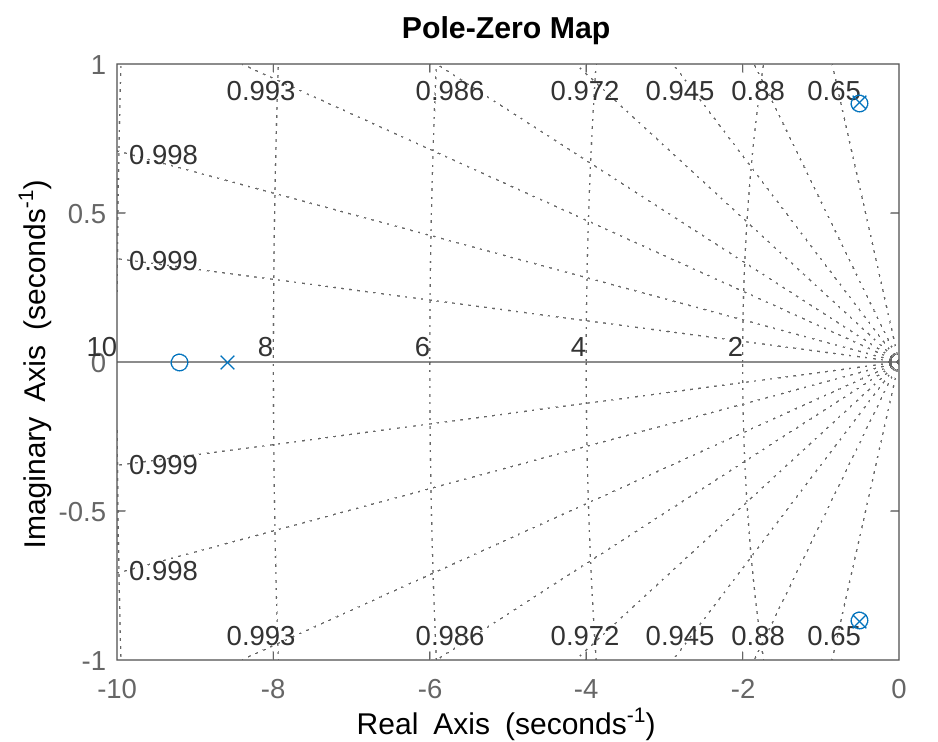
\includegraphics[scale=0.4]{Problem2Fig1.png}\\
As we can see, the poles all have their real parts less than 0, which means the system is stable.
\section*{Problem 3}
The blockdiagram for the nonlinear system looks like the following\\
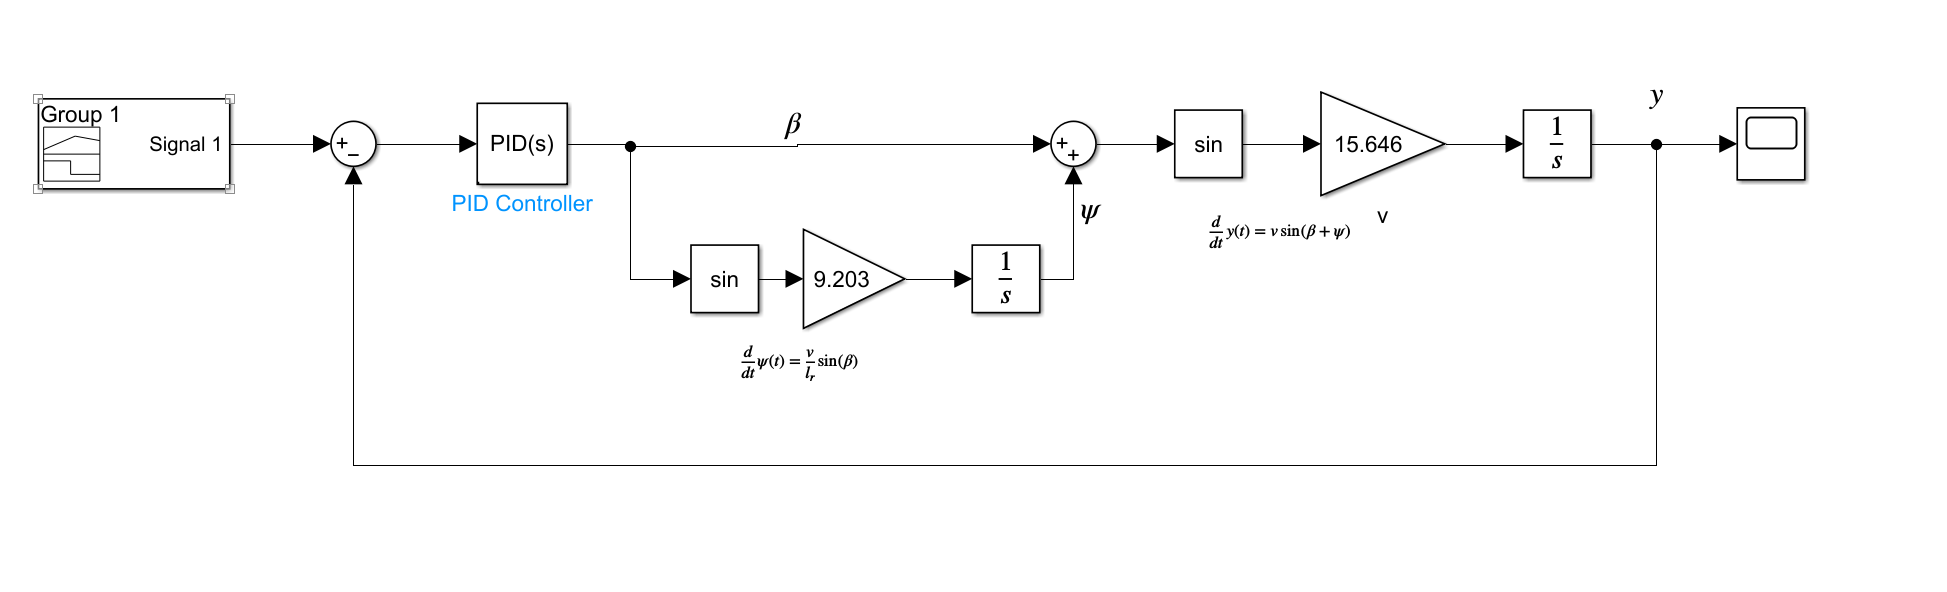
\includegraphics[scale=0.4]{Problem3BlockDiagram.PNG}\\
We can modify the inital conditions by modifying the inital conditions for the itegrator blocks. We define good behaviour such that the absolute value of $y$ is less than
$\frac{3.0-1.8}{2}=0.6$, ie the car cannot move out of its own line
\\\\
With the initial condition $y(0^+)=0.1$, and $\psi(0^+)=0$ the controller display's unacceptabl behavior, see the plot below.\\
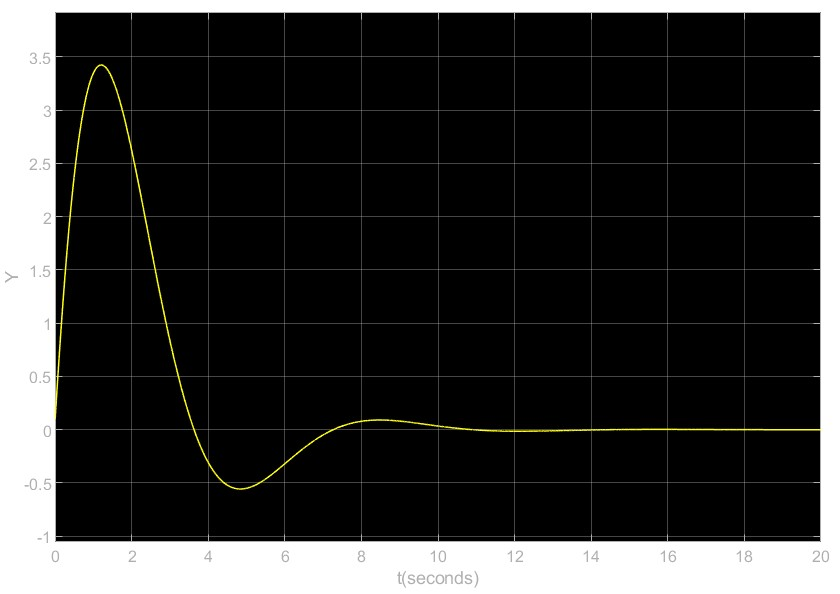
\includegraphics[scale=0.5]{Problem3y0.1psi0.jpg}\\
The car will initially move further away from $y=0$, reaching a max of around $y=3.5$ which is almost one lane away from the lane it needs to keep track off.

\end{document}